% !TeX root = main.tex


% Copyright 2014 by Emmanuel Boidot <eboidot3@gatech.edu>
\documentclass[10pt,compress]{beamer}

%%%% GT theme %%%%
% add 'gold' option for golden frame titles
% partToc (resp. sectionToc) creates table of contents at the beginning of each part (resp. section)
\usetheme[sectionToc,partToc]{GT} 
\usepackage{graphicx}
\usepackage[footnotesize]{subfigure}
\usepackage[english]{babel}
\usepackage[latin1]{inputenc}
\usepackage{hyperref}
\usepackage{siunitx}

\newcommand{\bs}[1]{\boldsymbol{#1}}
\newcommand{\D}[3]{\frac{\partial^{#1} #2}{\partial^{#1} #3}}
\newcommand{\tab}{\hspace{5mm}}
\newcommand{\tb}[1]{\textbf{#1}}

\usepackage{tcolorbox}
\usepackage{xcolor}



\title{Optimal Control for Nuclear Reactors}

% - Give the names in the same order as the appear in the paper.
% - Use the \inst{?} command only if the authors have different
%   affiliation.
\author[M. Louis]% (optional, appears in the lower left part of each frame)
{Calculus of Variations Final Presentation\texorpdfstring{\\}{}Matthew Louis}

\date{\today}


\begin{document}

{ % for the title frame, use the following options
\usebackgroundtemplate{\includegraphics[width=\paperwidth]{images/logos/Georgia-Tech-Insignia-Watermark-1200x1100}}
\setbeamertemplate{headline}{}
\setlength{\headheight}{0in}
\setbeamertemplate{footline}{}

% ----------
% Titlepage
% ----------

\begin{frame}
\titlepage
\end{frame}
}
\addtocounter{framenumber}{-1}


%%%%%%%%%%%%%%%%%%%%%%%%%%%%%%%%%%%%%%%% 
% \part[Intro]{Introduction} 

%%%%%
\begin{frame}\frametitle{Basics of Nuclear Power}
    \begin{enumerate}
        \item Just boils water to generate steam
        \item Energy released via fission chain reactions in fissile Uranium 235 (in fuel rods)
        \item Self-sustaining chain reaction that's stable due to negative feedback
    \end{enumerate}
    \begin{figure}
        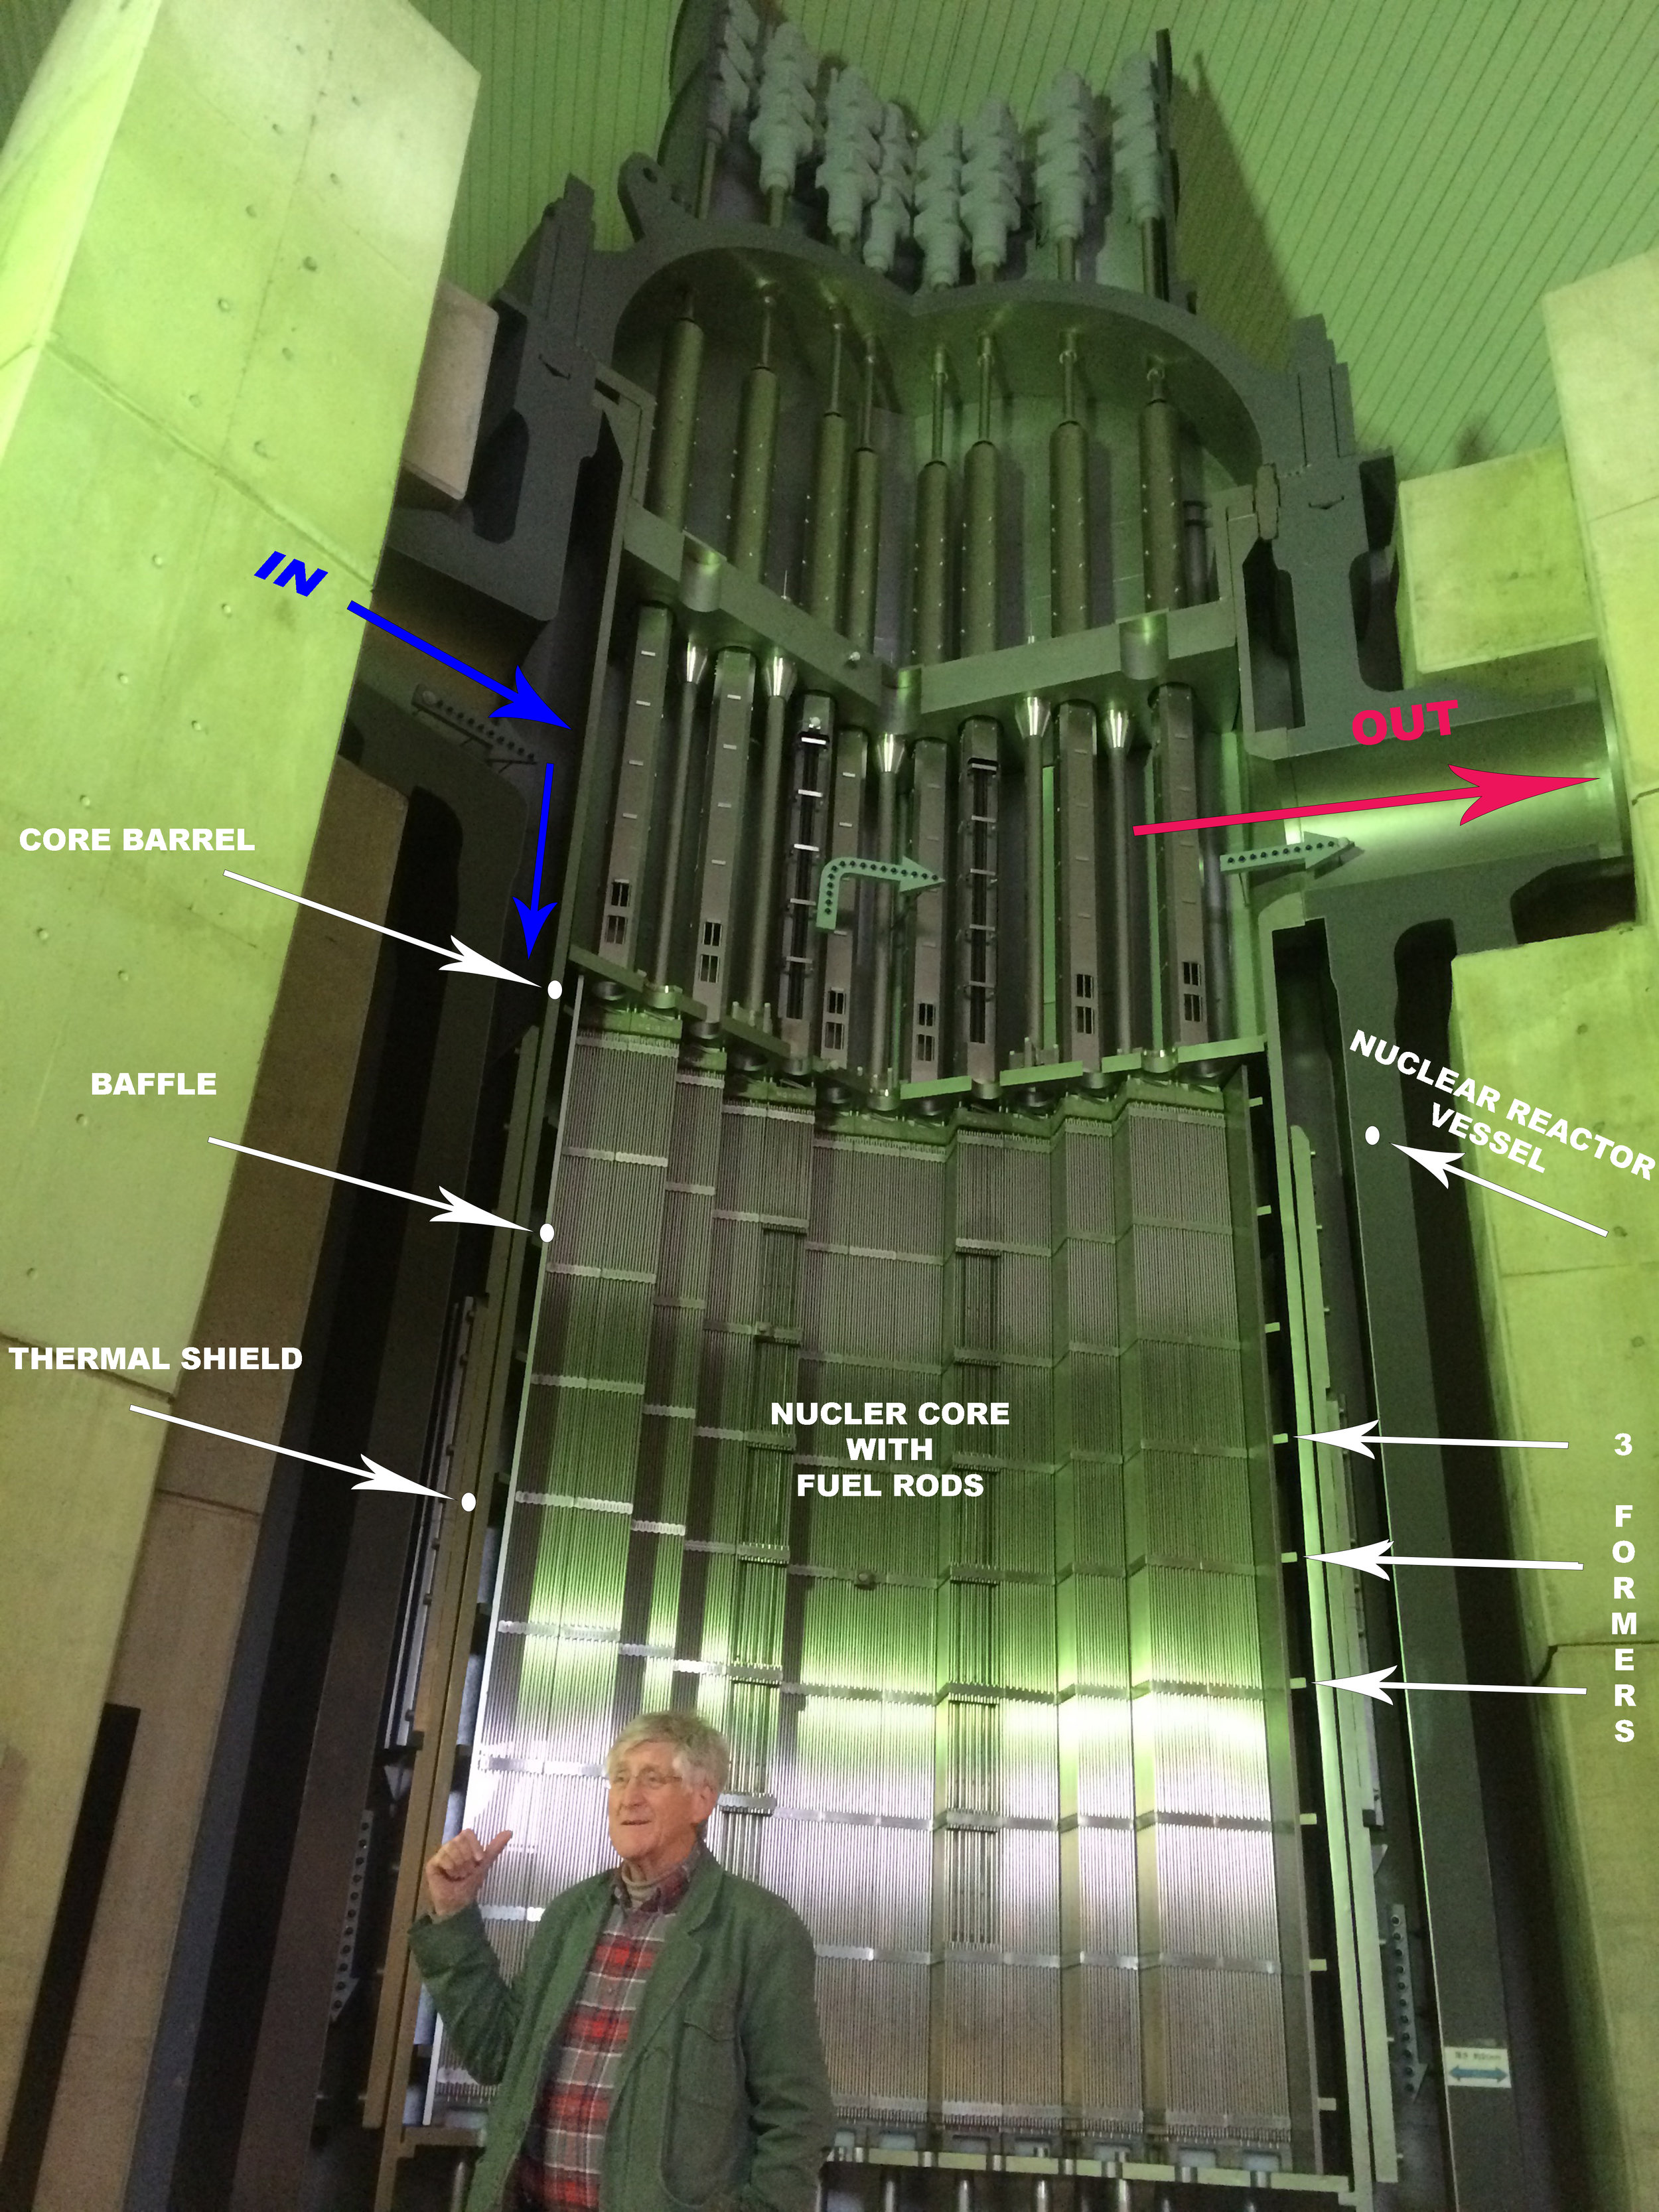
\includegraphics[width=0.4\textwidth]{images/core-cutaway.jpg}
    \end{figure}
\end{frame}


\begin{frame}\frametitle{Motivation}
We would like to understand how to best control the chain reaction to acheive a desired end state, e.g.
\begin{enumerate}
    \item Power uprate
    \item Reactor startup
    \item Minimize power peaking in the core
\end{enumerate}
Nominally operate at \emph{steady state}, but these state changes are necessarily \emph{dynamic}. 
Safety and performance relevant. Optimal control used historically to investigate these problems.

\begin{block}{Control Mechanisms}
In light water reactors (LWRs), there are two main control mechanisms
\begin{enumerate}
    \item Control rods: controlling \emph{rapid} changes in the chain reaction
    \begin{enumerate}
        \item Relevant for reactor dynamics
    \end{enumerate}
    \item Chemical shim: controlling \emph{slow} changes in in the chain reaction
\end{enumerate}
\end{block}

\begin{columns}

\end{columns}
\end{frame}

\begin{frame}\frametitle{Relevant Quantities in Reactor Physics}
Interested only in neutrons and their interations (fission, absorption, etc).
\begin{block}{Quantities}
    \begin{itemize}
        \item $\phi$ (the scalar flux): number of neutrons impinging on a cross sectional area per second.
        \item $\Sigma$ (the macroscopic cross section): characterizes the probabilitiy for a given interaction (measured in units of 1/L)
    \end{itemize}
\end{block}
\begin{block}{The Reaction Rate}
    With the scalar flux and the cross section, we can calculate reaction rates (e.g. of fission)
    \begin{equation}
        R_x = \Sigma_x \phi\nonumber
    \end{equation}
    units of \si{1/cm^3} (a reaction rate density), and subsequently the \emph{power}
    \begin{equation}
        P =``\int_V \Sigma_x \phi dV "\nonumber
    \end{equation}
\end{block}
\end{frame}

\begin{frame}\frametitle{Fission Chain Reactions and Controllability}
    \begin{block}{Controlling the Chain Reaction}
        The fission process is incredibly fast, and in a nuclear reactor, the time between a neutron's birth via fission and its next fission reaction is
        on the order of \si{\mu s}.
        \begin{enumerate}
            \item This would make controlling a reactor nearly impossible
            \item The response to small changes in the neutron multiplication factor result in \emph{extremely} rapid changes to power
        \end{enumerate}
    \end{block}
    \begin{block}{Prompt and Delayed Neutrons}
        During a fission event, some neutrons are released (nearly) immediately from the fissioning nucleus: \tb{prompt neutrons}, and some are emitted by subsequent decaay of
        fission products \tb{delayed neutrons}.
        \begin{flushleft}
        $\beta$: The fraction of fission neutrons that are delayed ($\approx 0.7\%$)
        \end{flushleft}
    \end{block}
\end{frame}

\begin{frame}\frametitle{Governing Equations}
Simplification of the general Boltzman equation from statistical mechanics
\begin{block}{The Linear Boltzman (Neutron Transport) Equation}
    State space $\bs{r}$, $\bs{\Omega}$, $E$, $t$ (or $\bs{r}$, $\bs{v}$, $t$) $\implies \psi(\bs{r}, \bs{\Omega}, E, t)$, the angular flux
    \begin{equation}
        \begin{split}
            \frac{1}{v}\D{}{\psi}{t} &= \hat{T}(t)\psi + \hat{F}_p(t) \int_{4\pi}\psi d\bs{\Omega} + \sum_{i=1}^6 \varepsilon_i(\bs{r}, E, t) - \hat{L}(t)\psi\\
            \D{}{\varepsilon_i}{t} &= -\lambda_i \varepsilon_i + \hat{F}_{d,i}\int_{4\pi}\psi d\bs{\Omega}\tab i=1,\cdots, 6
        \end{split}
    \end{equation}
\end{block}
\begin{block}{The Operators}
    All linear operators
    \begin{columns}
        \begin{column}{5cm}
            \begin{enumerate}
                \item $\hat{T}$: Scattering
                \item $\hat{F}_p$: Prompt fission
                \item $\hat{F}_d$: Delayed fission
            \end{enumerate}
        \end{column}
        \begin{column}{5cm}
            \begin{enumerate}
                \setcounter{enumi}{3}
                \item $\hat{L}$: Leakage
            \end{enumerate}
            Note that $\hat{F}_p + \hat{F}_d = \hat{F}_{tot}$
        \end{column}
    \end{columns}
\end{block}
\end{frame}

\begin{frame}\frametitle{The Factorization}
To derive a simplified model of the transport equation that's suitable for practical calculations, we need to \emph{factorize}.
\begin{block}{Motivation}
    The main idea is to separate the variation of the flux into a fast and slow component (due to delayed neutrons). Factorization of the form
    \begin{equation}
        \psi(\bs{r}, \bs{\Omega}, E, t)=A(t)\Psi(\bs{r}, \bs{\Omega}, E; t)\nonumber
    \end{equation}
    $A(t)$ called the \emph{amplitude} function and $\Psi(\bs{r}, \bs{\Omega}, E; t)$ the shape function.
\end{block}
This factorization is \emph{always} possible (not excluding any variables) and is not (yet) unique.
\end{frame}

\begin{frame}\frametitle{The Shape Equations}
    Substituting the factorization into the transport equation
    \begin{equation}
        \begin{split}
            &A(t)\frac{1}{v}\D{}{\Psi}{t} + \Psi \frac{1}{v}\frac{dA}{dt} \\
            &= A(t)\hat{T}(t)\Psi + A(t)\hat{F}_p(t) \int_{4\pi}\Psi d\bs{\Omega} + \sum_{i=1}^6 \varepsilon_i(\bs{r}, E, t) - A(t)\hat{L}(t)\Psi\nonumber\\
            \D{}{\varepsilon_i}{t} &= -\lambda_i \varepsilon_i + A(t)\hat{F}_{d,i}\int_{4\pi}\Psi d\bs{\Omega}\tab i=1,\cdots, 6
        \end{split}
    \end{equation}
    Called the shape equations, however, $A(t)$ is an unknown so as it stands these are not well-posed.
\end{frame}

\begin{frame}\frametitle{The Adjoint Equation}
    \begin{block}{The Reference Reactor}
        First define a reference reactor in steady state. The steady state problem is
        \begin{equation}
            \hat{L}_0(t)\psi_0=\hat{T}_0(t)\psi_0 +\frac{1}{k}\hat{F}_{tot,0}\int_{4\pi}\psi_0 d\bs{\Omega}\nonumber
        \end{equation}
        $k$ is a constant necessary for ensuring a solution exists. Physically it represents the neutron multiplication factor.
        For a critical reactor, $k=1$. Introduce the ``transport operator'' $\hat{H}_0$
        \begin{equation}
            (-\hat{L}_0 - \hat{T}_0 + \hat{F}_{tot,0})\psi_0 \equiv \hat{H}_0 \psi_0 =0\nonumber
        \end{equation}
    \end{block}
    \begin{block}{The Adjoint Equation}
        Define the inner product as the integral over the entire phase space (excluding $t$), then can define adjoint equation
        \begin{equation}
            \hat{H}_0^\dagger\psi_0^\dagger =0\nonumber
        \end{equation}
    \end{block}
\end{frame}

\begin{frame}\frametitle{Projecting Onto the Adjoint}
    $\psi_0^\dagger$ can be interpreted as an importance function.
    \begin{equation}
        \begin{split}
            &A(t)\braket{\psi_0^\dagger}{\frac{1}{v}\D{}{\Psi}{t}} + \braket{\psi_0^\dagger}{\frac{1}{v}\Psi} \frac{dA}{dt} \\
            &= A(t)\braket{\psi_0^\dagger}{\hat{T}(t)\Psi} + A(t)\braket{\psi_0^\dagger}{\hat{F}_p(t) \int_{4\pi}\Psi d\bs{\Omega}} + \cdots\\
            &+ \sum_{i=1}^6 \braket{\psi_0^\dagger}{\varepsilon_i(\bs{r}, E, t)} - A(t)\braket{\psi_0^\dagger}{\hat{L}(t)\Psi}\nonumber\\
            \braket{\psi_0^\dagger}{\D{}{\varepsilon_i}{t}} &= -\lambda_i \braket{\psi_0^\dagger}{\varepsilon_i} + A(t)\braket{\psi_0^\dagger}{\hat{F}_{d,i}\int_{4\pi}\Psi d\bs{\Omega}}\tab i=1,\cdots, 6
        \end{split}
    \end{equation}
\end{frame}

\begin{frame}\frametitle{Projecting Onto the Adjoint (Continued)}
    The adjoint ($\psi_0^\dagger$) is assumed constant in time, and so inner product and time derivatives can be interchanged.
    \begin{equation}
        \begin{split}
            &A(t)\D{}{}{t}\braket{\psi_0^\dagger}{\frac{1}{v}\Psi} + \braket{\psi_0^\dagger}{\frac{1}{v}\Psi} \frac{dA}{dt} \\
            &= A(t)\braket{\psi_0^\dagger}{\hat{T}(t)\Psi} + A(t)\braket{\psi_0^\dagger}{\hat{F}_p(t) \int_{4\pi}\Psi d\bs{\Omega}} + \cdots\\
            &+ \sum_{i=1}^6 \braket{\psi_0^\dagger}{\varepsilon_i(\bs{r}, E, t)} - A(t)\braket{\psi_0^\dagger}{\hat{L}(t)\Psi}\nonumber\\
            \D{}{}{t}\braket{\psi_0^\dagger}{\varepsilon_i} &= -\lambda_i \braket{\psi_0^\dagger}{\varepsilon_i} + A(t)\braket{\psi_0^\dagger}{\hat{F}_{d,i}\int_{4\pi}\Psi d\bs{\Omega}}\tab i=1,\cdots, 6
        \end{split}
    \end{equation}
\end{frame}

\begin{frame}\frametitle{Making the Factorization Unique}
    Since the factorization is not yet uniquely defined, we may make it uniquely defined by
    choosing the convenient condition
    \begin{equation}
        \D{}{}{t}\braket{\psi_0^\dagger}{\frac{1}{v}\Psi}=0\nonumber
    \end{equation}
    which allows us to eliminate the first term in the projected equations. If we divide each term by the quantity
    $\braket{\psi_0^\dagger}{\hat{F}_{tot,0}\Psi}$ (the importance of the fission neutrons distributed according to the shape $\Psi$).
    \begin{equation}
        \begin{split}
            \frac{\braket{\psi_0^\dagger}{\frac{1}{v}\Psi}}{\braket{\psi_0^\dagger}{\hat{F}_{tot,0}\Psi}} \frac{dA}{dt} &= A(t)\frac{\braket{\psi_0^\dagger}{(\hat{T}(t)-\hat{L}(t) + \hat{F}_p(t))\Psi}}{\braket{\psi_0^\dagger}{\hat{F}_{tot,0}\Psi}} +\sum_{i=1}^6\frac{ \braket{\psi_0^\dagger}{\varepsilon_i(\bs{r}, E, t)}}{\braket{\psi_0^\dagger}{\hat{F}_{tot,0}\Psi}} \nonumber\\
            \D{}{}{t}\frac{\braket{\psi_0^\dagger}{\varepsilon_i}}{\braket{\psi_0^\dagger}{\hat{F}_{tot,0}\Psi}} &= -\lambda_i \frac{\braket{\psi_0^\dagger}{\varepsilon_i}}{\braket{\psi_0^\dagger}{\hat{F}_{tot,0}\Psi}} + A(t)\frac{\braket{\psi_0^\dagger}{\hat{F}_{d,i}\int_{4\pi}\Psi d\bs{\Omega}}}{\braket{\psi_0^\dagger}{\hat{F}_{tot,0}\Psi}}\tab i=1,\cdots, 6
        \end{split}
    \end{equation}
\end{frame}

\begin{frame}\frametitle{The Physical Interpretations}
    \begin{itemize}
        \item \begin{flushleft}
            The effective generation time of prompt neutrons
            \begin{equation}
                \Lambda(t)=\frac{\braket{\psi_0^\dagger}{\frac{1}{v}\Psi}}{\braket{\psi_0^\dagger}{\hat{F}_{tot,0}\Psi}}\nonumber
            \end{equation}
        \end{flushleft}
        \item \begin{flushleft}
            The Reactivity (related to the multiplication factor)
            \begin{equation}
                \rho(t)=\frac{\braket{\psi_0^\dagger}{\hat{H}(t)\Psi}}{\braket{\psi_0^\dagger}{\hat{F}_{tot,0}\Psi}}\nonumber
            \end{equation}
        \end{flushleft}
        \item \begin{flushleft}
            The effective delayed neutron fraction for the $i$th group
            \begin{equation}
                \tilde{\beta}_i(t)=\frac{\braket{\psi_0^\dagger}{\hat{F}_{d,i}\Psi}}{\braket{\psi_0^\dagger}{\hat{F}_{tot,0}\Psi}}\nonumber
            \end{equation}
        \end{flushleft}
    \end{itemize}
\end{frame}

\begin{frame}\frametitle{The Physical Interpretations (Continued)}
    \begin{itemize}
        \item \begin{flushleft}
            The total effective delayed neutron fraction
            \begin{equation}
                \tilde{\beta}(t) = \sum_{i=1}^6 \tilde{\beta}_i(t)\nonumber
            \end{equation}
        \end{flushleft}
        \item \begin{flushleft}
            The total effective delayed neutron emission for the $i$th group
            \begin{equation}
                \tilde{C}_i(t)=\frac{\braket{\psi_0^\dagger}{\varepsilon_i(t)}}{\braket{\psi_0^\dagger}{\hat{F}_{tot,0}\Psi}}\nonumber
            \end{equation}
        \end{flushleft}
    \end{itemize}
    Using these parameters, we can rewrite the projected equations
    \begin{equation}
        \begin{split}
            \frac{dA(t)}{dt} &= \frac{\rho(t)- \tilde{\beta}(t)}{\Lambda(t)}A(t) + \sum_{i=1}^6\lambda_i \tilde{C}_i(t)\nonumber\\
            \D{}{}{t}\tilde{C}_i(t) &= -\lambda_i \tilde{C}_i(t) + \frac{\tilde{\beta}_i(t)}{\Lambda(t)}A(t)\tab i=1,\cdots, 6
        \end{split}
    \end{equation}
\end{frame}

\begin{frame}\frametitle{The Point Kinetic Model}
    \begin{itemize}
        \item The above system of equation has a nonlinear coupling through the shape function
        \item Very hard to solve
        \item A simplified model can be obtained by neglecting spatial dependence
    \end{itemize}
    Assuming that
    \begin{equation}
        \begin{split}
            \Psi(\bs{r}, \bs{\Omega}, E;t) \approx \Psi(\bs{r}, \bs{\Omega}, E;t=0) &= \psi_0(\bs{r}, \bs{\Omega}, E)\nonumber\\
            A(t=0)&=1
        \end{split}
    \end{equation}
    The coefficients in the shape equation become constants. Usually rescale the equations so that $A(t)\to P(t)$ i.e. the total power.
    \begin{block}{The Point Kinetic Equations}
        \begin{equation}
            \begin{split}
                \frac{dP(t)}{dt} &= \frac{\rho- \tilde{\beta}}{\Lambda}P(t) + \sum_{i=1}^6\lambda_i \tilde{C}_i(t)\nonumber\\
                \D{}{}{t}\tilde{C}_i(t) &= -\lambda_i \tilde{C}_i(t) + \frac{\tilde{\beta}_i}{\Lambda}P(t)\tab i=1,\cdots, 6
            \end{split}
        \end{equation}
    \end{block}
\end{frame}

\begin{frame}\frametitle{Feedback}

\end{frame}

\begin{frame}\frametitle{Description of the State Space}

\end{frame}

\begin{frame}\frametitle{Example Optimal Control Problems}

\end{frame}

\begin{frame}\frametitle{References}

\end{frame}

\end{document}